\documentclass{article}
\usepackage{url}
\usepackage{tabularx}
\usepackage{amssymb}
\usepackage{amsmath}
\usepackage[margin=1in]{geometry}
\usepackage[nottoc]{tocbibind}
\usepackage{graphicx}
\usepackage{adjustbox}
\usepackage{float}
\usepackage{changepage}
\graphicspath{ {./img/} }

\title{STAT UN2103 Homework 6}
\author{
  Jackson Chen
  \and
  jc4697
}
\date{\today}

\begin{document}
  \maketitle

  \section{Introduction}

    The purpose of this project is to conduct analysis on data containing a variety
    demographic factors regarding wages. More specifically, the aim is to determine
    a model with worker demographics as the covariates and the wage as a response variable.
    The model is supposed to correlate the input data as much as possible, so that the
    model would be able to be an effective predictive tool for wages. Creating a more
    realistic model also allows us to examine the larger research question surrounding
    this project, which is as follows:
    \begin{quote}
      Do African Americans have statistically different wages compared to Caucasian males?
      How do their wages also statistically compare all other males?
    \end{quote}

    The covariates included in the data consist of years of education (\texttt{edu}),
    job experience (\texttt{exp}), college graduate (\texttt{deg}), working in or near a city
    (\texttt{city}), US region (\texttt{reg}), commuting distance (\texttt{com}), number
    of employees in a company (\texttt{emp}), and race (\texttt{race}).

    In order to effectively train a model and test it, the input data was split into
    a training and a validation set. The validation data set had 4965 entries, or about
    $20\%$ of the input dataset. The training set consisted of the remaining $80\%$ of
    the rows. A quality assurance check was then done on the split sets in order to assure
    relative heterogeneity of the datasets.

    Exploratory data analysis was conducted on the training dataset. The process will be
    described in the following sub-sections.

    \subsection{Preliminary Model Investigation}


  \section{Statistical Model} \label{final_model}

  \section{Research Question}

  \section{Appendix}
    This section contains the exact process that led to the determination of the final
    model described in Section \ref{final_model}. This process can be broken into two steps:
    The selection, transformation, and interaction of the covariates that created the
    final model, and the validation of the final model against a range of diagnostic tools.

    \subsection{Model Selection}
      The first step in the exploratory data analysis consisted of creating new columns in the
      data frame to map the categorical string variables \texttt{deg, city, reg, race} into
      numeric categorical variables. The purpose of this step is to satisfy the signature for \texttt{R}'s \texttt{I()}
      function, which groups covariates together into an interaction variable.

      After the training-validation split was done on the data, a QQ plot was plotted on
      the untransformed dataset, as shown in Figure \ref{fig:qqwage}. However the end
      of the QQ plot had too extreme of a vertical gradient. Therefore a logarithmic
      transformation would reduce the extremity at this end. Figure \ref{fig:qqlogwage}
      shows the QQ plot on the logarithmically transformed response variable. The
      overall structure of the points as well as the end behavior are much more
      normal.

      \begin{figure}
        \centering
        \begin{minipage}{.45\textwidth}
          \centering
          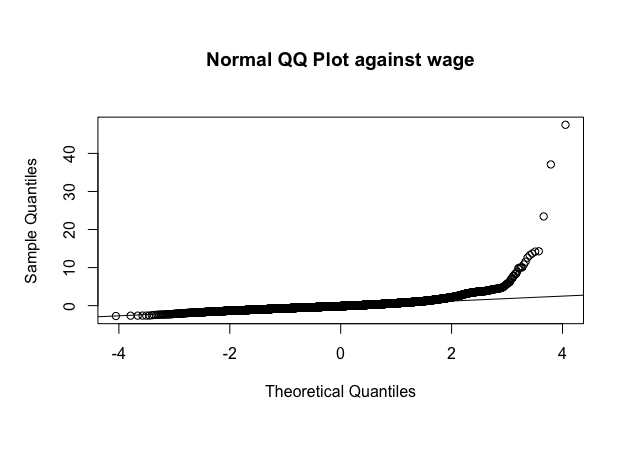
\includegraphics[scale=0.35]{qqwage}
          \caption{QQ plot on untransformed wage}
          \label{fig:qqwage}
        \end{minipage}
        \begin{minipage}{.45\textwidth}
          \centering
          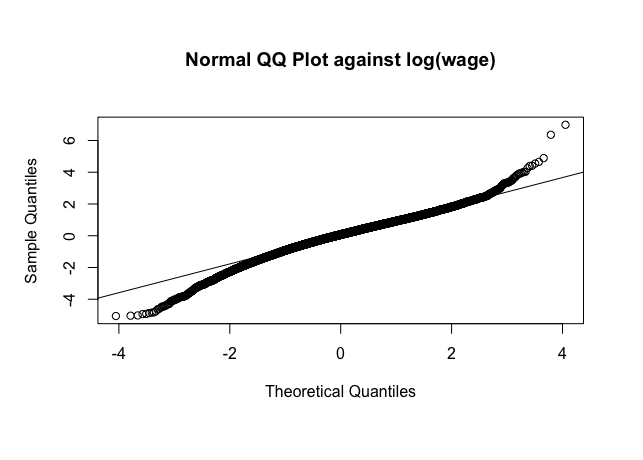
\includegraphics[scale=0.35]{qqlogwage}
          \caption{QQ plot on log transformed wage}
          \label{fig:qqlogwage}
        \end{minipage}
      \end{figure}

      The next step involved verifying whether each of the covariates in the input dataset
      actually correlated with \texttt{wage}. This purpose was this was to determine
      which variables to investigate further in terms of transformations, functional forms,
      and interactions. The more formal process for eliminating covariates occurs in the
      reduction of explanatory variables stage.

      From Figure \ref{fig:scattercom}, it appears that the commute time has no impact
      on wages. This is determined visually by examining that the linear smoothing of the graph
      has no gradient and thus indicates no relationship. We can verify this more numerically
      by running a marginal t-test on a linear model between the wages and the commute time.
      The null hypothesis in this test would be $\beta_1 = 0$, with the commute time
      as the $x_1$ term. The p value is 0.79 and is greater than the 0.05 significance
      cutoff, indicating the failure to reject the null hypothesis.

      On the other hand, the other covariates show an existent relationship with wages
      (or the log of the wage). Figures \ref{fig:scatterexp} to \ref{fig:boxrace} provide
      graphical support behind such claims. Only a select number of covariates were displayed
      since the graphs behind the other covariates follow a very similar trend. By
      observing the smoothing functions for all of the aforementioned graphs,
      one can determine the transformations necessary to construct the
      most predictive linear model with respect to wages. Most of the smoothing
      functions indicate a somewhat linear path indicating a strict linear relationship,
      with one exception.

      Figure \ref{fig:scatterexp} depicts a downward-facing
      quadratic relationship between the number of years of experience and the log
      of the wages. Upon further inspection, Figure \ref{fig:boxexp} represents
      the relationship more clearly with the inner quartile ranges following the
      same quadratic trend. Therefore, \texttt{exp} requires a quadratic transformation
      to resolve this violation in linearity. \\


      At this stage of the analysis, we have determined that the model will have
      a logarithmically transformed response variable \texttt{wage} and a quadratically
      transformed covariate \texttt{exp}. The last important component of the model
      now needs to be examined: interactions between covariates. This analysis will
      consist of three parts:
      \begin{enumerate}
        \item Interactions among categorical variables
        \item Interactions between categorical and continuous variables
        \item Interactions among continuous variables
      \end{enumerate}

      

      \begin{figure}
        \centering
        \begin{minipage}{.45\textwidth}
          \centering
          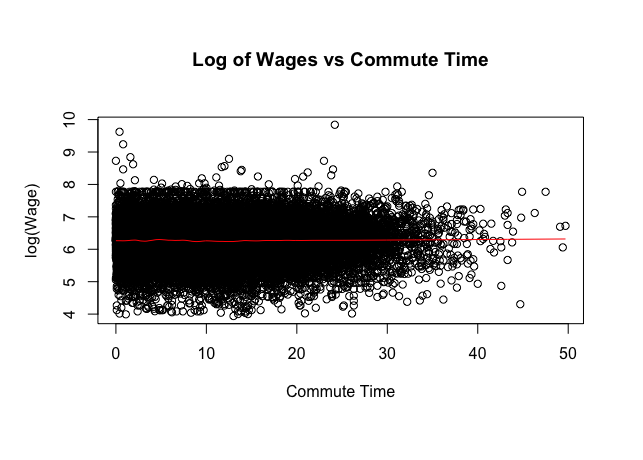
\includegraphics[scale=0.35]{scattercom}
          \caption{Scatter plot on commute time}
          \label{fig:scattercom}

          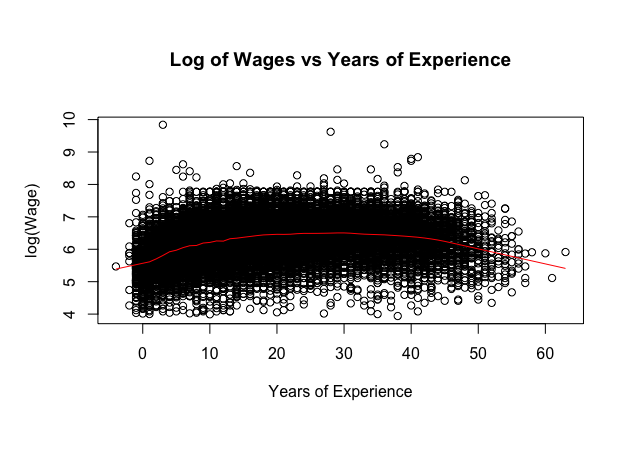
\includegraphics[scale=0.35]{scatterexp}
          \caption{Scatter plot on years of experience}
          \label{fig:scatterexp}

          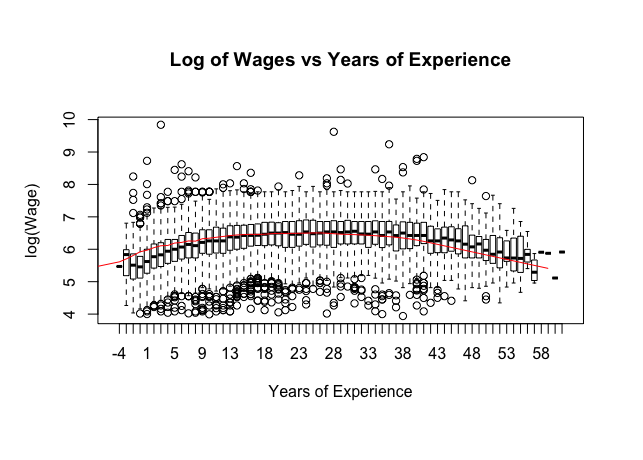
\includegraphics[scale=0.35]{boxexp}
          \caption{Box plot on years of experience}
          \label{fig:boxexp}
        \end{minipage}
        \begin{minipage}{.45\textwidth}
          \centering
          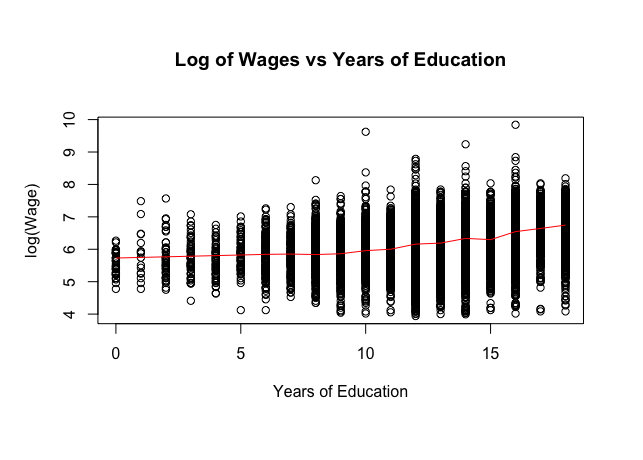
\includegraphics[scale=0.35]{scatteredu}
          \caption{Scatter plot on number of employees}
          \label{fig:scatteredu}

          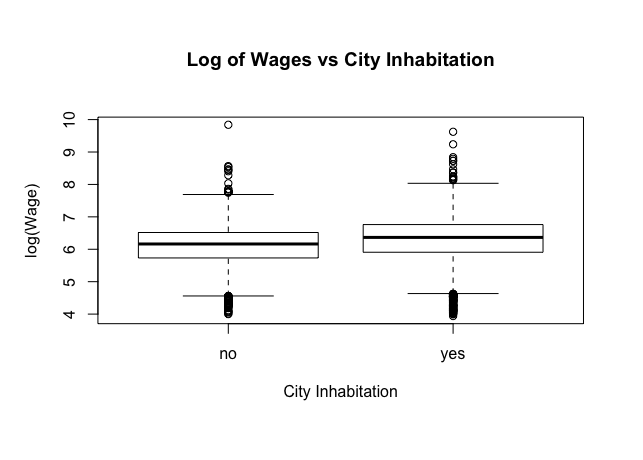
\includegraphics[scale=0.35]{boxcity}
          \caption{Scatter plot on number of employees}
          \label{fig:boxcity}

          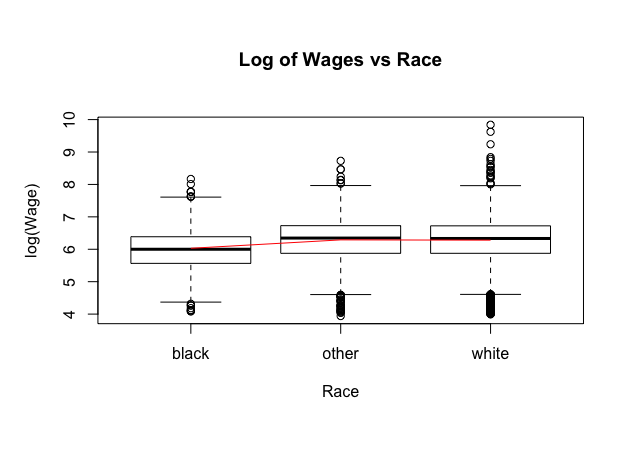
\includegraphics[scale=0.35]{boxrace}
          \caption{Scatter plot on number of employees}
          \label{fig:boxrace}
        \end{minipage}
      \end{figure}

    \subsection{Diagnostics and Model Validation}

    \subsection{Additional Notes}
\end{document}
